\documentclass[compress]{beamer}

\mode<presentation>
{
  %\usetheme{Warsaw}
  %\usecolortheme{spruce}
  % or ...
	%\useoutertheme{infolines}
  %\setbeamercovered{transparent}
  
  \usetheme{CambridgeUS}
    \setbeamercolor{item projected}{bg=darkred}
    \setbeamertemplate{enumerate items}[default]
    \setbeamertemplate{navigation symbols}{}
    \setbeamercovered{invisible}
    \setbeamercolor{block title}{fg=darkred}
    \setbeamercolor{local structure}{fg=darkred}
  
  % or whatever (possibly just delete it)
}

\usepackage{verbatim} 
\usepackage{listings}
\usepackage{tikz}
\usetikzlibrary{arrows.meta}
\usetikzlibrary{shapes}
\tikzstyle{block}=[draw opacity=0.7,line width=1.4cm]

\definecolor{darkgreen}{RGB}{50,171,24}

\newcommand{\bigpause}{\bigskip \pause}

\lstloadlanguages{C++}
\lstnewenvironment{code}
	{%\lstset{	numbers=none, frame=lines, basicstyle=\small\ttfamily, }%
	 \csname lst@SetFirstLabel\endcsname}
	{\csname lst@SaveFirstLabel\endcsname}
\lstset{% general command to set parameter(s)
	language=C++, basicstyle=\footnotesize\sffamily, keywordstyle=\slshape,
	emph=[1]{tipo,usa}, emphstyle={[1]\sffamily\bfseries},
	basewidth={0.47em,0.40em},
	columns=fixed, fontadjust, resetmargins, xrightmargin=5pt, xleftmargin=15pt,
	flexiblecolumns=false, tabsize=2, breaklines,	breakatwhitespace=false, extendedchars=true,
	numbers=left, numberstyle=\tiny, stepnumber=1, numbersep=9pt,
	frame=l, framesep=3pt,
}

\usepackage[spanish]{babel}
% or whatever

\usepackage[utf8]{inputenc}
% or whatever

\usepackage{times}
\usepackage[T1]{fontenc}
% Or whatever. Note that the encoding and the font should match. If T1
% does not look nice, try deleting the line with the fontenc.


\title[Camino mínimo en grafos] % (optional, use only with long paper titles)
{Camino mínimo en grafos}

\author[Melanie Sclar] % (optional, use only with lots of authors)
{~Melanie Sclar}
% - Give the names in the same order as the appear in the paper.
% - Use the \inst{?} command only if the authors have different
%   affiliation.
\institute[UBA] % (optional, but mostly needed)
{
  %\inst{1}%
  Facultad de Ciencias Exactas y Naturales\\
  Universidad de Buenos Aires
}
\date[Nacional OIA 2016] % (optional, should be abbreviation of conference name)
{Nacional OIA 2016}

% Ac¿ se puede insertar el logo de la UBA
% \pgfdeclareimage[height=0.5cm]{university-logo}{university-logo-filename}
% \logo{\pgfuseimage{university-logo}}



% Delete this, if you do not want the table of contents to pop up at
% the beginning of each subsection:
\AtBeginSubsection[]
{
  \begin{frame}<beamer>{Contenidos}
    \tableofcontents[currentsection,currentsubsection]
  \end{frame}
}

\newcommand{\be}{\begin{equation*}}
\newcommand{\ee}{\end{equation*}}
\newcommand{\state}[1]{\left|\,#1\,\right\rangle}
\newcommand{\costate}[1]{\left\langle\,#1\,\right|}
\newcommand{\trace}{\text{Tr}}
\newcommand{\su}{\uparrow}
\newcommand{\sd}{\downarrow}
\newcommand{\im}{\text{Im}}
\newcommand{\re}{\text{Re}}

% If you wish to uncover everything in a step-wise fashion, uncomment
% the following command:

%\beamerdefaultoverlayspecification{<+->}


\begin{document}
\pgfdeclarelayer{background}
\pgfsetlayers{background,main}
\begin{frame}
  \titlepage
\end{frame}

\section{Camino mínimo}
\subsection{Introducción}
\begin{frame}
Esta charla tratará sobre uno de los problemas más renombrados de la
computación: \textbf{el problema del camino mínimo}. Este problema 
consiste en hallar la mejor forma de ir desde un punto a otro (o a varios
otros) minimizando la distancia recorrida, el tiempo invertido, entre
varias posibilidades.

\bigskip
\bigskip

Es un problema muy útil en las olimpíadas, pero no solamente aquí.
Veamos dos ejemplos de la vida real que deben resolver el problema que
trataremos hoy.
\end{frame}


\begin{frame}{Camino m\'inimo}
\begin{center}
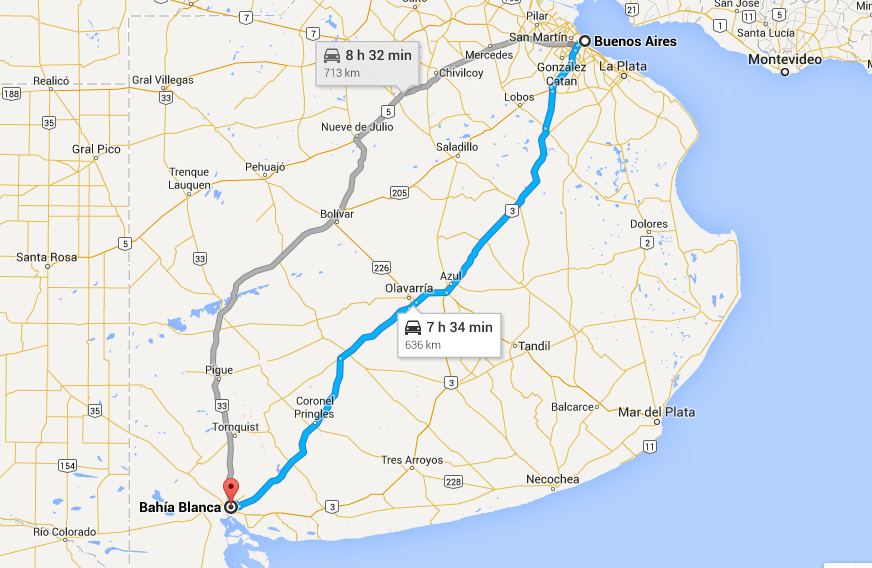
\includegraphics[height=7cm]{google-maps.png} \\
\end{center}
\end{frame}

\begin{frame}{Camino m\'inimo}
\begin{center}
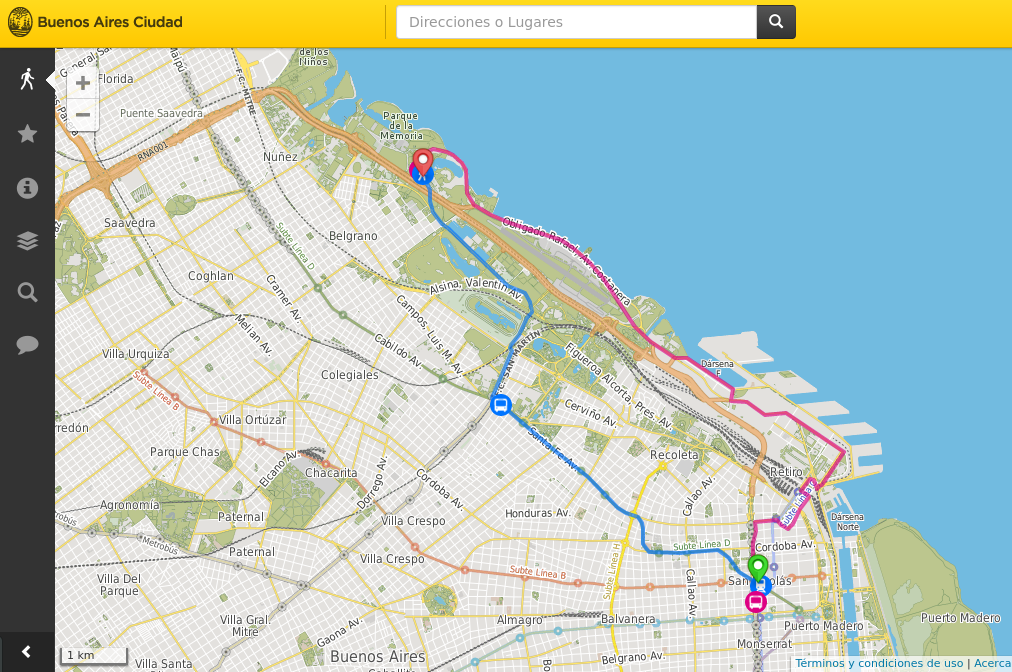
\includegraphics[height=7cm]{mapa-buenos-aires.png} \\
\end{center}
\end{frame}

\begin{frame}{Representando el problema}
Para poder resolver estos problemas debemos poder representarlos de manera
concisa y abstracta, desprendiéndonos de las particularidades de cada
caso de uso posible.

\bigskip

La representación más usual de este tipo de problemas (ya sea para aplicarlo
en problemas de camino mínimo o no) es la de \textbf{grafos}.
\end{frame}

\subsection{Representación con grafos}
\begin{frame}{\textquestiondown Qué es un grafo?}
\begin{exampleblock}{}
  {\large ``Un grafo es un conjunto, no vacío, de objetos llamados vértices 
  (o nodos) y una selección de pares de vértices, llamados aristas 
  (edges en inglés) que pueden ser orientados (dirigidos) o no.''}
  \vskip5mm
  \hspace*\fill{\small--- Wikipedia}
\end{exampleblock}
  \pause
\invisible<1>{
\begin{exampleblock}{}
  {\large ``Un grafo es un conjunto de puntos y líneas que unen pares de esos puntos''}
  \vskip5mm
  \hspace*\fill{\small--- La Posta}
\end{exampleblock}

}
\end{frame}

\begin{frame}{Grafos dirigidos y no dirigidos}

{\small
En los grafos no dirigidos las aristas son doble mano (se puede ir en ambos sentidos). \\
En los dirigidos en cambio, las aristas se recorren en un único sentido: desde el origen al destino de la flecha. Si queremos representar que la calle que une las esquinas $u$ y $v$ es doble mano deberemos poner dos aristas: una que vaya de $u$ a $v$ y otra que vaya de $v$ a $u$.}

\begin{center}
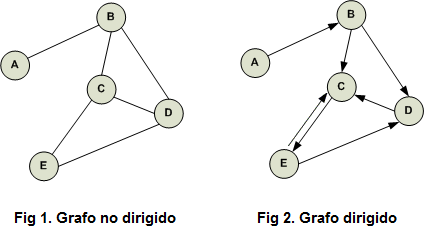
\includegraphics[scale=0.75]{grafos-dirigidos-y-no-dirigidos.png}
\end{center}
\end{frame}

\begin{frame}{\textquestiondown Para qué podemos usar los grafos?}
Mediante un grafo podemos representar, por ejemplo, una ciudad. Las esquinas serían los vértices y las conexiones por medio de una calle entre dos esquinas serían los ejes. Si todas las calles son doble mano, el grafo es no dirigido.
Si algunas calles son mano única el grafo es dirigido: ¿cómo modelamos una calle doble mano aquí?

\bigskip
A medida que los problemas se dificultan, puede suceder que sea difícil que a uno se le ocurra modelar el problema con un grafo, pero que una vez que lo hayamos hecho, el problema se vuelva sencillo utilizando los algoritmos que veremos hoy. 

\end{frame}

\begin{frame}
De ahora en más trabajaremos con grafos no dirigidos por simplicidad, pero también podrían aplicarse a grafos dirigidos.

\begin{block}{Vecindad}
Diremos que dos nodos son $adyacentes$ o $vecinos$ si existe una arista que los une.
\end{block}

\begin{block}{Distancia}
La distancia entre dos nodos $u$ y $v$ es la mínima cantidad de ejes por los que me tengo que mover para salir de $u$ y llegar a $v$. Si hay múltiples formas de llegar de $u$ a $v$, me quedo con la más corta.
\end{block}

\end{frame}

\begin{frame}{Formas de representar un grafo}
Existen varias maneras de guardar un grafo en memoria para poder luego consultar cosas (por ejemplo, recorrer el grafo, que es lo que haremos hoy).

Veamos las dos más populares.
\end{frame}

\begin{frame}{Matriz de adyacencia}
\begin{block}{Matriz de adyacencia}
La matriz de adyacencia es una matriz de $n \times n$ donde $n$ es la cantidad de nodos del grafo, que en la posición ($i,j$) tiene un 1 (o true) si hay una arista entre los nodos $i$ y $j$ y 0 (o false) si no.
\end{block}

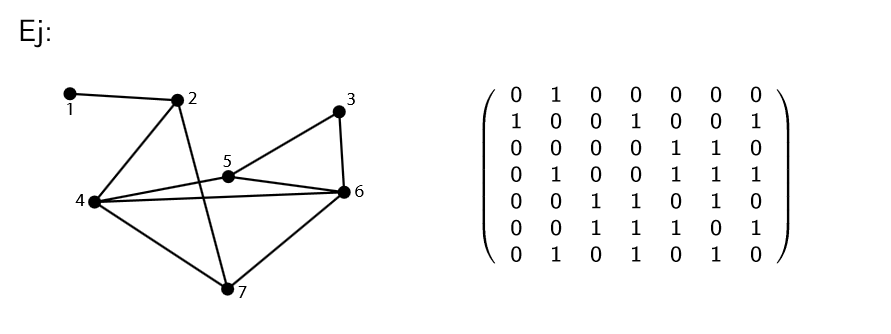
\includegraphics[scale=0.5]{matriz-adyacencia.png}
\end{frame}

\begin{frame}{Matriz de adyacencia}
Esta es una de las representaciones m\'as utilizadas. Si bien el ejemplo es para un grafo no dirigido, tambi\'en se puede utilizar la misma estructura para grafos dirigidos y grafos con pesos.
\bigskip

{\bf Ventajas}
\pause
\invisible<1> {
	\begin{itemize}
		\item Permite saber si existe o no arista entre dos nodos cualesquiera en O(1).
		\item Es muy f\'acil de implementar, $matrizAdy[i][j]$ guarda toda la informaci\'on sobre la arista.
	\end{itemize}
}
\bigpause
{\bf Desventajas}
\pause
\invisible<1> {
	\begin{itemize}
		\item La complejidad espacial: se necesitan $n^2$ casillas para representar un grafo de $n$ nodos.
	\end{itemize}
}
\end{frame}

\begin{frame}{Lista de adyacencia}
\begin{block}{Lista de adyacencia}
La lista de adyacencia es un vector de vectores de enteros, que en el $i$-ésimo vector tiene el número $j$ si hay una arista entre los nodos $i$ y $j$.
\end{block}

Coloquialmente la llamamos {\it lista de vecinos} pues para cada nodo guardamos la lista de nodos para los que existe una arista que los conecta (o sea, los vecinos).
\bigskip
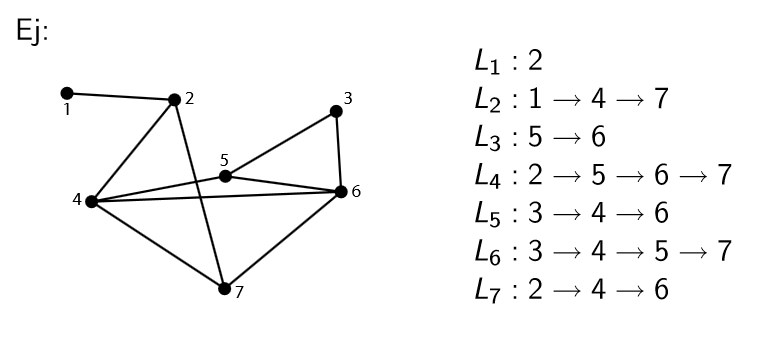
\includegraphics[scale=0.5]{lista-vecinos.png}
\end{frame}

\begin{frame}{Lista de adyacencia}
Nuevamente, con la misma idea tambi\'en se pueden modelar grafos dirigidos y con pesos.\bigskip

La complejidad espacial de esta representaci\'on ser\'a posiblemente mucho menor. ?`Cu\'anta memoria necesitaremos para un grafo de $n$ nodos y $m$ aristas? \pause {\bf O(m+n)}
\end{frame}

\begin{frame}{Formalización del problema de camino mínimo}

Precisemos mejor nuestro problema, usando los términos de grafos que
acabamos de aprender.

\begin{block}{Problema de Camino m\'inimo}
Dado un grafo $G$ con pesos en las aristas, el problema de
camino mínimo entre dos nodos $u$ y $v$ consiste en encontrar un camino
entre esos nodos cuyo peso sea menor o igual que el peso de cualquier
otro camino entre $u$ y $v$.
\end{block}

\bigskip

Según qué tipo de grafo analicemos, la solución al problema será diferente.
Por ejemplo, si el grafo no tuviera pesos (o si todos los pesos fueran iguales,
que a efectos prácticos es lo mismo), nos conviene usar otro algoritmo (BFS).

\end{frame}

\subsection{Algoritmo de Dijkstra}
\begin{frame}{Algoritmo de Dijkstra}
Este algoritmo fue creado por uno de los padres de la computación,
Edger W. Dijkstra, en 1956. Sirve para cualquier grafo con pesos (dirigido
o no) \textbf{siempre y cuando sus pesos no sean negativos}.

\bigskip

El algoritmo calcula las distancias mínimas desde un nodo inicial a todos 
los demás. Para hacerlo, en cada paso se toma el nodo más cercano al inicial
que aún no fue visitado. Por ser el más cercano aún no visto, esta distancia
que hallamos es la mínima (reflexionaremos más sobre esto). Así, en cada
paso tenemos un subconjunto de nodos que están bien resueltos, y con cada
iteración agregaremos un nodo más a nuestro conjunto, hasta resolver el 
problema en su totalidad.

\bigskip

Veamos un ejemplo.
\end{frame}


\begin{frame}{Algoritmo de Dijkstra - Ejemplo}

\begin{pgfpicture}{0cm}{0cm}{11cm}{7cm}
	\pgfsetlinewidth{1pt}
	\pgfnodecircle{v1}[stroke]{\pgfxy(2,3)}{2mm}			
	\pgfputat{\pgfxy(2,3)}{\pgfbox[center,center]{1}}
	\pgfnodecircle{v2}[stroke]{\pgfxy(4,5)}{2mm}
	\pgfputat{\pgfxy(4,5)}{\pgfbox[center,center]{2}}
	\pgfnodecircle{v3}[stroke]{\pgfxy(7,5)}{2mm}
	\pgfputat{\pgfxy(7,5)}{\pgfbox[center,center]{3}}
	\pgfnodecircle{v4}[stroke]{\pgfxy(9,3)}{2mm}
	\pgfputat{\pgfxy(9,3)}{\pgfbox[center,center]{4}}
	\pgfnodecircle{v5}[stroke]{\pgfxy(7,1)}{2mm}
	\pgfputat{\pgfxy(7,1)}{\pgfbox[center,center]{5}}
	\pgfnodecircle{v6}[stroke]{\pgfxy(4,1)}{2mm}
	\pgfputat{\pgfxy(4,1)}{\pgfbox[center,center]{6}}
	\pgfnodesetsepend{3pt}
	\pgfsetarrowsend{Triangle[scale=0.7pt]}
    \pgfnodeconnline{v1}{v2}
	\pgfnodeconnline{v1}{v6}			
	\pgfnodeconnline{v1}{v3}			
	\pgfnodelabel{v1}{v2}[0.5][5pt]{\pgfbox[center,center]{4}}			
	\pgfnodeconnline{v2}{v3}
	\pgfnodelabel{v2}{v3}[0.5][5pt]{\pgfbox[center,center]{3}}						
	\pgfnodeconnline{v3}{v4}
	\pgfnodelabel{v3}{v4}[0.5][5pt]{\pgfbox[center,center]{1}}						
	\pgfnodeconnline{v5}{v4}
	\pgfnodelabel{v5}{v4}[0.5][5pt]{\pgfbox[center,center]{4}}						
	\pgfnodeconnline{v6}{v5}			
	\pgfnodelabel{v6}{v5}[0.5][5pt]{\pgfbox[center,center]{3}}			
	\pgfnodelabel{v1}{v6}[0.5][5pt]{\pgfbox[center,center]{3}}			
	\pgfnodelabel{v1}{v3}[0.5][5pt]{\pgfbox[center,center]{7}}			
	\pgfnodeconnline{v2}{v5}			
	\pgfnodelabel{v2}{v5}[0.5][5pt]{\pgfbox[center,center]{1}}			
	\pgfnodeconnline{v3}{v5}			
	\pgfnodelabel{v3}{v5}[0.5][5pt]{\pgfbox[center,center]{1}}			
	
	\onslide<2-2>{
		\pgfputat{\pgfxy(5,7)}{\pgfbox[left,top]{$\pi=(0,\infty,\infty,\infty,\infty,\infty)$}}
	}
	\onslide<2-3>{
		\pgfputat{\pgfxy(1,7)}{\pgfbox[left,top]{$S=\{1\}$}}
	}
	
	\color{orange}
	\onslide<2->{
		\pgfnodecircle{v1}[stroke]{\pgfxy(2,3)}{2mm}			
	}
	
	\color{black}
	\onslide<3-5>{
	   \pgfputat{\pgfxy(5,7)}{\pgfbox[left,top]{$\pi=(0,4,7,\infty,\infty,3)$}}
	}
	
	\onslide<3->{
		\color{darkgreen}
		\pgfnodeconnline{v1}{v2}
		\pgfnodeconnline{v1}{v6}			
		\pgfnodeconnline{v1}{v3}
	}
	
	\color{black}
	\onslide<4-6>{
		\pgfputat{\pgfxy(1,7)}{\pgfbox[left,top]{$S=\{1,6\}$}}
	}
	
	\color{orange}
	\onslide<4->{
		\pgfnodecircle{v6}[stroke]{\pgfxy(4,1)}{2mm}			
		\pgfnodeconnline{v1}{v6}			
	}
	
	\color{blue}
	\onslide<5-5>{
		\pgfnodeconnline{v6}{v5}
	}
	
	\color{black}
	\onslide<6-8>{
	  \pgfputat{\pgfxy(5,7)}{\pgfbox[left,top]{$\pi=(0,4,7,\infty,6,3)$}}
	}
	
	\color{darkgreen}
	\onslide<6-8>{
		\pgfnodeconnline{v6}{v5}
	}
	
	\color{black}		
	\onslide<7-9>{
		\pgfputat{\pgfxy(1,7)}{\pgfbox[left,top]{$S=\{1,6,2\}$}}
	}
	
	\color{orange}
	\onslide<7->{
		\pgfnodecircle{v2}[stroke]{\pgfxy(4,5)}{2mm}			
		\pgfnodeconnline{v1}{v2}
	}
	
	\color{blue}
	\onslide<8-8>{
		\pgfnodeconnline{v2}{v3}
		\pgfnodeconnline{v2}{v5}
	}
	
	\color{darkgreen}
	\onslide<9-11>{
		\pgfnodeconnline{v2}{v5}
		\color{black}
		\pgfputat{\pgfxy(5,7)}{\pgfbox[left,top]{$\pi=(0,4,7,\infty,5,3)$}}
	}
	
	\color{black}
	\onslide<10-12>{
		\pgfputat{\pgfxy(1,7)}{\pgfbox[left,top]{$S=\{1,6,2,5\}$}}
	}

	\color{orange}
	\onslide<10->{
		\pgfnodecircle{v5}[stroke]{\pgfxy(7,1)}{2mm}			
		\pgfnodeconnline{v2}{v5}
	}
	
	\color{blue}
	\onslide<11-11>{
		\pgfnodeconnline{v5}{v4}
	}
	
	\color{black}
	\onslide<12-14>{
		\pgfputat{\pgfxy(5,7)}{\pgfbox[left,top]{$\pi=(0,4,7,9,5,3)$}}
		\color{darkgreen}
		\pgfnodeconnline{v5}{v4}
	}
	
	\color{black}
	\onslide<13-15>{
		\pgfputat{\pgfxy(1,7)}{\pgfbox[left,top]{$S=\{1,6,2,5,3\}$}}
	}

	\color{orange}
	\onslide<13->{
		\pgfnodecircle{v3}[stroke]{\pgfxy(7,5)}{2mm}			
		\pgfnodeconnline{v1}{v3}
	}
	
	\color{blue}
	\onslide<14-14>{
		\pgfnodeconnline{v3}{v4}
	}
	
	\color{black}
	\onslide<15->{
		\pgfputat{\pgfxy(5,7)}{\pgfbox[left,top]{$\pi=(0,4,7,8,5,3)$}}
		\color{darkgreen}
		\pgfnodeconnline{v3}{v4}
	}
	
	\onslide<16->{
	  \color{black}
		\pgfputat{\pgfxy(1,7)}{\pgfbox[left,top]{$S=\{1,6,2,5,3,4\}$}}
	}

	\color{orange}
	\onslide<16->{
		\pgfnodecircle{v4}[stroke]{\pgfxy(9,3)}{2mm}			
		\pgfnodeconnline{v3}{v4}
	}
\end{pgfpicture}
\end{frame}



\begin{frame}[fragile]{Pseudocódigo de Dijkstra sin cola de prioridad}
\begin{lstlisting}
Dijkstra (Grafo G, nodo inicial s)
  visitado[n] = {false, ..., false} // guarda si un nodo ya fue visitado
  distancia[n] = {Infinito, ..., Infinito} // guarda las distancias del nodo salida al resto
  
  para cada w en V[G] hacer
     si existe arista entre s y w entonces
         distancia[w] = peso (s, w)

  distancia[s] = 0
  visitado[s] = true
  
  mientras que no esten visitados todos hacer 
     v = nodo de menor distancia a s que no fue visitado aun
     visitado[v] = true
     para cada w en sucesores (G, v) hacer
         si distancia[w] > distancia[v] + peso (v, w) entonces
            distancia[w] = distancia[v] + peso (v, w)

\end{lstlisting}
\end{frame}

\begin{frame}[fragile]{Pseudocódigo de Dijkstra con cola de prioridad}
\begin{lstlisting}
Dijkstra (Grafo G, nodo_fuente s)       
   para todo u en V[G] hacer
       distancia[u] = INFINITO
       padre[u] = NULL
       visitado[u] = false
       
   distancia[s] = 0
   adicionar (cola, (s, distancia[s]))
   
   mientras que cola no sea vacia hacer
       u = extraer_minimo(cola)
       visitado[u] = true
       para todo v en adyacencia[u] hacer
           si no visitado[v] y distancia[v] > distancia[u] + peso (u, v) hacer
              distancia[v] = distancia[u] + peso (u, v)
              padre[v] = u
              adicionar(cola,(v, distancia[v]))
\end{lstlisting}
\end{frame}

\subsection{Camino mínimo en una grilla}
\begin{frame}
Puntos principales:
Vector de movimientos
Representar una dirección y un giro
Bordes

\end{frame}

\section{Árbol generador mínimo}
\subsection{Algoritmo de Prim}
\begin{frame}

\end{frame}

\begin{frame}
\begin{center}
{\Huge \textquestiondown Preguntas?}
\end{center}
\end{frame}

\end{document}
